%%%%%%%%%%%%%%%%%%%%%%%%%%%%%%%%%%%%%%%%%%%%%%%%
% E.Pinault-Bigeard - e.pinault-bigeard@upsti.fr
% http://s2i.pinault-bigeard.com
% CC BY-NC-SA 2.0 FR - http://creativecommons.org/licenses/by-nc-sa/2.0/fr/
%%%%%%%%%%%%%%%%%%%%%%%%%%%%%%%%%%%%%%%%%%%%%%%%
\documentclass[11pt]{article}
%%%%%%%%%%%%%%%%%%%%%%%%%%%%%%%%%%%%%%%%%%%%%%%%
% Package UPSTI_Document
%%%%%%%%%%%%%%%%%%%%%%%%%%%%%%%%%%%%%%%%%%%%%%%%
%%%%%%%%%%%%%%%%%%%%%%%%%%%%%%%%%%%%%%%%%%%%%%%%
% Package UPSTI_Document
%%%%%%%%%%%%%%%%%%%%%%%%%%%%%%%%%%%%%%%%%%%%%%%%
\usepackage{subcaption}
\usepackage[usenames, svgnames, dvipsnames]{xcolor}
\usepackage{UPSTI_Document}
\usepackage{pgfplots}
\usepackage{import}
\definecolor{darkspringgreen}{rgb}{0.09, 0.45, 0.27}

\newcommandx*{\dessinRepereFigGeo}[5][1=\vx{},2=\vy{},3=\vz{},4=,5=0]
	{
		\draw [->,very thick] (0,0) -- (1,0) ;
		\draw [->,very thick] (0,0) -- (0,1) ;
    \fill[white] (0,0) circle (0.13);
    \draw [->,very thick] (0,0) circle (0.13);
    \ifnumequal{#5}{0} {% z vers nous
      \fill[black] (0,0) circle (0.03);
      \draw [->,thick] (0,0) circle (0.04);
    }{% z vers la feuille
  		\begin{scope} [rotate=45]
  			\draw [-,thick] (0,-0.12) -- (0,0.12) ;
  			\draw [-,thick] (-0.12,0) -- (0.12,0) ;
  		\end{scope}
    }
		\draw [anchor=north west] (1.1,0) node {${#1}$};
		\draw [anchor=south west] (0,1.1) node {${#2}$};
		\draw [anchor=north east] (-0.1,0) node {${#3}$};
		\draw [anchor=north west] (-0.1,-0.1) node {${#4}$};
	}

	\usepackage{array}
	\newcolumntype{L}[1]{>{\raggedright\let\newline\\\arraybackslash\hspace{0pt}}m{#1}}
	\newcolumntype{C}[1]{>{\centering\let\newline\\\arraybackslash\hspace{0pt}}m{#1}}
	\newcolumntype{R}[1]{>{\raggedleft\let\newline\\\arraybackslash\hspace{0pt}}m{#1}}

	\usepackage{pifont}% http://ctan.org/pkg/pifont
\newcommand{\cmark}{\color{green}\ding{51}}%
\newcommand{\xmark}{\color{red}\ding{55}}%
\newcommand{\fmark}{\ding{229}}%
\newcommand{\itemc}{\item[\cmark]}%
\newcommand{\itemx}{\item[\xmark]}%
\newcommand{\itemf}{\item[\fmark]}%


\usetikzlibrary[circuits.plc.ladder]            %     
\newlength{\ladderskip}\setlength{\ladderskip}{5\tikzcircuitssizeunit}%5\tikzcircuitssizeunit    = 355pt
\newlength{\ladderrungsep}
\setlength{\ladderrungsep}{.2\ladderskip}
\def\ladderrungend#1{\pgftransformyshift{-#1\ladderskip-\ladderrungsep}}

%---------------------------------%
% Paramètres du package
%---------------------------------%

% Version du document (pour la compilation)
% 1: Document prof
% 2: Document élève
% 3: Document à publier
\newcommand{\UPSTIidVersionDocument}{2}


% Classe
% 1: PTSI				6: PSI*			11: TSI2		16: Spé
% 2: PT	(par défaut)	7: MPSI			12: ATS
% 3: PT*				8: MP			13: PC
% 4: PCSI				9: MP*			14: PC*
% 5: PSI				10: TSI1		15: Sup
%\newcommand{\UPSTIidClasse}{2}



% Matière
% 1: S2I (par défaut)    2: IPT     3: TIPE
% 6: Vie au lycée
\newcommand{\UPSTIvariante}{5}
\newcommand{\UPSTIidMatiere}{0}
\newcommand{\UPSTIintituleMatiere}{Automatique}
\newcommand{\UPSTIsigleMatiere}{Autom}
% Type de document
% 0: Custom*				7: Fiche Métho de			14: Document Réponses
% 1: Cours (par défaut)		8: Fiche Synthèse    		15: Programme de colle
% 2: TD     				9: Formulaire
% 3: TP						10: Memo
% 4: Colle					11: Dossier Technique
% 5: DS						12: Dossier Ressource
% 6: DM						13: Concours Blanc
% * Si on met la valeur 0, il faut décommenter la ligne suivante:
%\newcommand{\UPSTItypeDocument}{Custom}
\newcommand{\UPSTIidTypeDocument}{1}

% Titre dans l'en-tête


% Titre dans l'en-tête

\newcommand{\UPSTIvariante}{5}

\newcommand{\UPSTItitreEnTete}{Automatisme industriel}
%\newcommand{\UPSTItitreEnTetePages}{}
\newcommand{\UPSTIsousTitreEnTete}{Introduction aux API}


% Titre
%\newcommand{\UPSTItitrePreambule}{Automatisme industriel}
\newcommand{\UPSTItitre}{La programmation d'un Automate Industriel}

% Durée de l'activité (pour DS, DM et TP)
\newcommand{\UPSTIduree}{3h30}

% Note de bas de première page
%\newcommand{\UPSTInoteBasDePremierePage}{Geoffrey Vaquette}
% Numéro (ajoute " n°1" après DS ou DM)
\newcommand{\UPSTInumero}{2}

% Numéro chapitre
%\newcommand{\UPSTInumeroChapitre}{1}

% En-tête customisé
%\newcommand{\UPSTIenTetePrincipalCustom}{UPSTIenTetePrincipalCustom}

% Message sous le titre
%\newcommand{\UPSTImessage}{Message sous le titre}


% Référence au programme
%\newcommand{\UPSTIprogramme}{\EPBComp \EPBCompP{B1-02}, \EPBCompP{B2-49}, \EPBCompS{B2-50}, \EPBCompS{B2-51}, \EPBCompP{C1-07}, \EPBCompP{C1-08}}

% Si l'auteur n'est pas l'auteur par défaut
%\renewcommand{\UPSTIauteur}{WWOOOOOOWW}

% Si le document est réalisé au nom de l'équipe
%\newcommand{\UPSTIdocumentCollegial}{1}

% Source
\newcommand{\UPSTIsource}{G. Vaquette, H. Discours}

% Version du document
\newcommand{\UPSTInumeroVersion}{2.1}

%-----------------------------------------------
\UPSTIcompileVars		% "Compile" les variables
%%%%%%%%%%%%%%%%%%%%%%%%%%%%%%%%%%%%%%%%%%%%%%%%


%%%%%%%%%%%%%%%%%%%%%%%%%%%%%%%%%%%%%%%%%%%%%%%%
% Début du document
%%%%%%%%%%%%%%%%%%%%%%%%%%%%%%%%%%%%%%%%%%%%%%%%
\begin{document}
\UPSTIbuildPage

%\UPSTIobjectif{Durant cette activité, nous allons analyser une trame pour l'envoi d'informations sur une étiquette.}

\tableofcontents

\pagebreak

\section{Premières machines à état}
\subsection{Application du cours : Tableau mobile}
\begin{UPSTIactivite}
    \UPSTIquestion{Implémenter la machine à état du tableau de classe sous la forme d'un circuit logique}
    \UPSTIquestion{Vérifier son fonctionnement en simulation}
\end{UPSTIactivite}

\subsection{Une divergence en OU}
On désire implémenter le fonctionnement suivant : 

\UPSTIboiteCentrale{Cahier des charges}{
    Soit un système avec trois boutons $B_p1$, $B_p2$ et $B_p3$
    \begin{enumerate}
        \item Sur l'écran du logo, au départ il est écrit \textit{Bonjour à tous !} sur fond blanc
        \item Ensuite, selon le bouton activé : 
        \begin{description}
            \item[$B_p1$ : ] Affichage du message \textit{Sortez vite !} sur fond rouge
            \item[$B_p2$ : ] Affichage du message \textit{Rentrez vite !} sur fond orange 
        \end{description}
        \item Ensuite, un appui sur $B_p3$ remet le système à l'état initial
    \end{enumerate}
}

\begin{UPSTIactivite}
    \UPSTIquestion{Dessiner la machine à état correspondante}
    \vspace{5cm}
    \UPSTIquestion{Implémenter cette machine à état sur LogoSoft}
\end{UPSTIactivite}
\UPSTIpresenceProf{Faire une démonstration du bon fonctionnement des deux programmes à un enseignant}


\section{Moteur pas à pas}
\subsection{Présentation}
On met à votre disposition un moteur pas à pas.
Ce moteur est constitué de 4 enroulements (bobines) appelée phases et repérées par un numéro (0, 1, 2, 3). On désire commander chacune de ces phases par une sortie de l’automate (Q0.0, Q0.1, Q0.2, Q0.3). 

Il existe de multiples façons pour commander les phases du moteur, pour le TP nous allons utiliser une commande très simple, dont le principe de fonctionnement est détaillé ci-dessous : 

\begin{minipage}{.6\textwidth}
    Le rotor, constitué d’un aimant, se place face à la bobine qui
est alimentée (une seule phase est commandée à la fois).
En commandant successivement chacune des bobines, le
rotor se déplace de bobine en bobine, vers celle qui est
nouvellement alimentée (Voir Figure~\ref{fig:pasApas}). Dans la réalité le moteur comporte
beaucoup plus que 4 positions par tour, mais la séquence de
commande 0-2-1-3, sera la même pour faire déplacer le
rotor de pas en pas.
\end{minipage}\hfill
\begin{minipage}{.35\textwidth}
    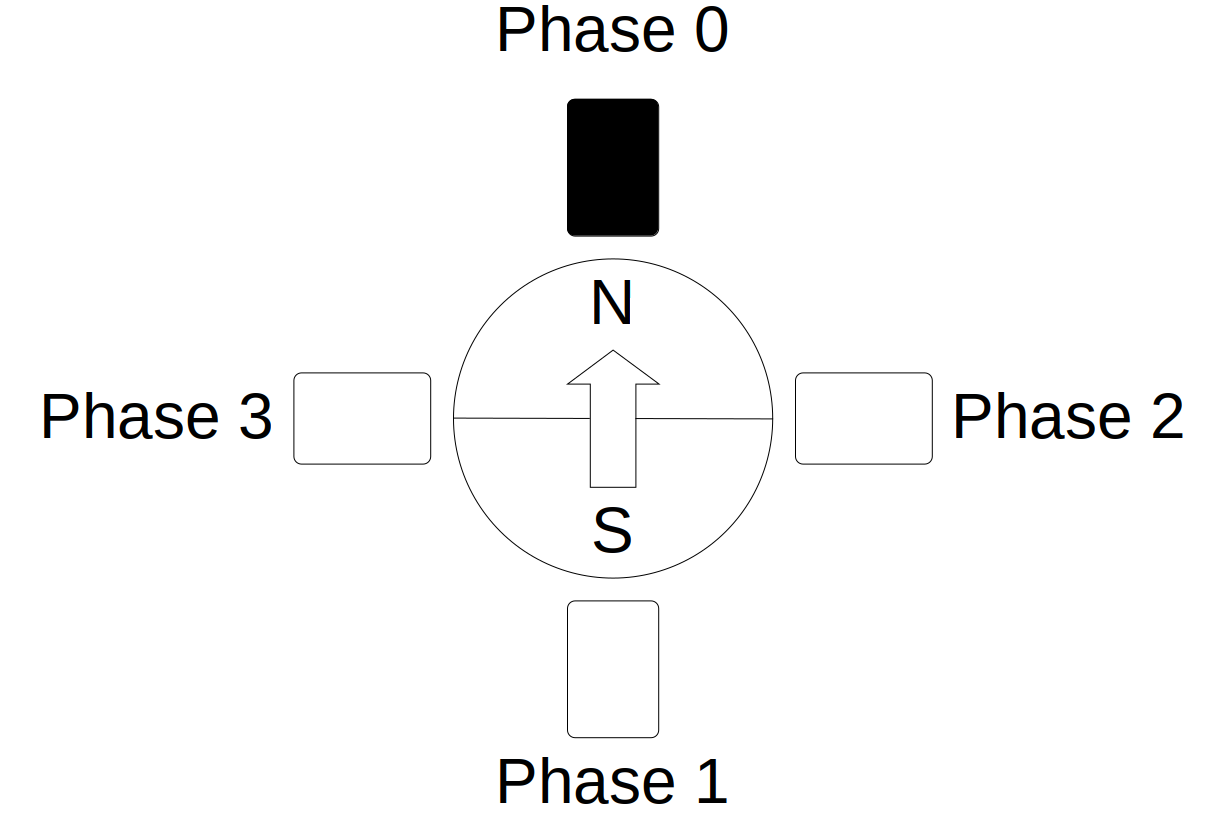
\includegraphics[width=\textwidth]{images/pasAPas_01.png}
\end{minipage}


\begin{figure}[h]
    \centering
    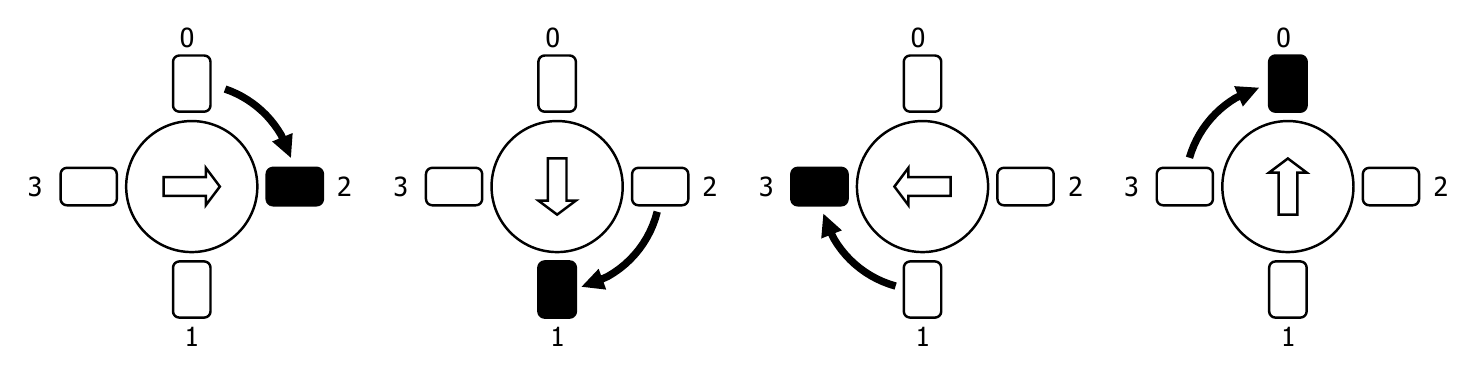
\includegraphics[width=.8\textwidth]{images/pasAPas_02.png}
    \caption{Schéma de principe d'un moteur pas à pas}
    \label{fig:pasApas}
\end{figure}

\subsection{Travail à effectuer}


\begin{UPSTIactivite}
    \UPSTIquestion{A partir de la lecture du fonctionnement présenté ci-dessus, dessiner la machine à état permettant la rotation du moteur pas à pas}
    \vspace{6cm}
\end{UPSTIactivite}

\begin{UPSTIactivite}
    \UPSTIquestion{Implémenter ce fonctionnement en circuit logique}
\UPSTIquestion{Câbler le moteur pas à pas sur la maquette}
\UPSTIquestion{Vérifier le bon fonctionnement}
\end{UPSTIactivite}

\UPSTIattention{Attention, il existe différents modèles de moteurs pas à pas. Demander à votre enseignant de vous expliquer les rôles des différents câbles présents}

\UPSTIboiteCentrale{Cahier des charges : Rotation du moteur pas à pas}{
    \begin{itemize}
        \item Un mémento à \SI{5}{Hz} cadence la séquence décrite en Figure~\ref{fig:pasApas}
        \item Un appui sur $B_p0$ Stoppe le moteur qui restera figé dans sa position
        \item Un appui sur $B_p7$ coupe l'alimentation des bobines et remet le système à son état initial
        \item Les bobines ne sont pas alimentées tant que $B_p7$ est actif
    \end{itemize}
}

\begin{UPSTIactivite}
    \UPSTIquestion{Compléter la machine à état pour respecter le cahier des charges}
    \UPSTIquestion{Implémenter ces modifications}
\end{UPSTIactivite}

\begin{UPSTIactivite}
    \UPSTIquestion{Modifier la machine à état pour un changement de sens après appui sur $B_p1$}
    \UPSTIquestion{Ajouter un choix de vitesse (faible ou élevée) à l'aide du $B_p2$}
    \UPSTIquestion{Ajouter une variable qui compte le nombre de pas réalisés. Cette variable sera remise à 0 lors de l'initialisation par le $B_p7$}
\end{UPSTIactivite}

\begin{UPSTIactivite}
    \UPSTIquestion{Associer la rotation du moteur au codeur incrémental fourni par l'enseignant}

    Dans cette configuration, l'horloge n'est plus fournie par un mémento cadencé mais par les impulsions fournies par le codeur.
\end{UPSTIactivite}




\end{document}
